\documentclass[../../main.tex]{subfiles}

%-----------------------------------------------------------%
\begin{document}
\section{Estimation}
{

\subsection{Introduction}
{
Attitude of a satellite refers to its orientation in space with respect to some reference frame. Attitude determination is the process of finding three independent quantities, which are necessary for any minimal parameterization of the attitude. There is a very subtle difference between attitude determination and attitude estimation. Attitude determination in the strictest sense refers to the memory-less approaches that determine the attitude point-by-point in time, quite often without taking the statistical properties of the attitude measurements into account. Attitude estimation, on the other hand, refers to approaches with memory, i.e. those that use a dynamic model of the spacecraft’s motion in a filter that retains information from a series of measurements taken over time. For our system, we are doing Attitude determination.

The inputs to the algorithm are a set of inertial frame vectors of the image stars that have been identified by the star-matching algorithm.The corresponding body-frame vectors of those stars are also the inputs to the estimator block. Since star catalogues generally follow ICRF(International Celestial Reference Frame) coordinate system, the inertial frame vectors will be in ICRF and thus the determined attitude will be with respect to ICRF. The output of the algorithm is the estimated quaternion, which is equivalent to the attitude matrix from inertial frame to the body frame.
}

\subsection{Estimation Algorithms}  
{

\subsubsection{TRIAD Algorithm}
{
The name \textbf{``TRIAD"} is an acronym for \textbf{TRIaxial Attitude Determination}. This spacecraft attitude determination method uses exactly two vector measurements i.e. for star trackers, measurements from only two stars would be used. In a star tracker we have more number of measurements available but the algorithm is incapable of utilising more than 2. Therefore TRIAD is not a preferred choice for a star tracker.
}


\subsubsection{AIM Algorithm}
\label{sec:AIM}
{
 \textbf{AIM} is an acronym for \textbf{Attitude estimation using Image Matching}.
Almost all the attitude estimation algorithms are based on the minimisation of Wahba's loss function(discussed in later sections). These attitude estimation algorithms all share one important drawback, when used with a star tracker. They
determine the attitude of the spacecraft, based on observations which are represented as unit vectors. In a
star tracker however, the observations are 2D star centroids on the image plane. The conversion of these 2D
coordinates to unit vectors is not straightforward. Because of optical and electronic distortion, temperature,
magnetic and star intensity effects, an empirical model based on laboratory calibrations is usually used
to convert the coordinates.\newline
AIM is another algorithm that was looked into during literature survey. We choose QUEST algorithm for our system as it is the most commonly used algorithm for star trackers and has a long history of successful applications. 

}


\subsubsection{Wahba's Problem}
{
We can improve on the TRIAD method in two ways: by allowing arbitrary weighting
of the measurements and by allowing the use of more than two measurements. The latter is especially important for use with star trackers that can track many stars simultaneously.Wahba’s problem is to find the orthogonal matrix A with determinant 1 that minimizes the loss function:
\begin{equation}
    L(A)=\frac{1}{2} \sum_{i=1}^{n}a_{i}||b_{i}-Ar_{i}||^2
\end{equation}
where $b_i$ is a set of n unit vectors measured in spacecraft's body frame, $r_i$ are the corresponding unit vectors in a reference frame, and $a_i$ are non-negative
weights.

Algorithms for solving Wahba’s problem fall into two classes. The first solves for the attitude matrix directly, and the second solves for the quaternion representation of the attitude matrix. Matrix solutions of Wahba's problem include \textbf{Singular Value Decomposition method}, \textbf{Fast Optimal Attitude matrix(FOAM)} etcetra. Quaternion solutions include \textbf{Davenport's q method}, \textbf{QUEST}, \textbf{ESOQ} etcetra. Quaternion solutions have proven to be much useful in practice. Among the above mentioned algorithms QUEST is most popularly used for star trackers. The AIM algorithm mentioned before uses 2-D vectors instead of 3-D and thus has a different cost function.

Using the orthogonality of A, the unit norm of the vectors and the cyclic invariance of trace:
\begin{equation}
||b_{i}-Ar_{i}||^2 = ||b_{i}||^2 + ||Ar_{i}||^2 -2b_{i}.(Ar_{i}) = 2- 2 tr(Ar_{i}b_{i}^{T})
\end{equation}
Thus we can write the cost function as:
\begin{equation}
    L(A)= \lambda _{0} - tr(AB^{T})
\end{equation}
with
\begin{equation}
    \lambda_{0}= \sum_{i=1}^{n} a_{i}
\end{equation}

and the Attitude profile matrix B defined as 
\begin{equation}
    B= \sum_{i=1}^{n} a_{i} b_{i} r_{i}^{T}
\end{equation}
Now it is clear that the loss function is minimised when tr(A$B^T$) is maximised.

}



}

\subsection{QUEST}
{
\subsubsection{QUEST 1}
{
Using the quaternion representation of attitude matrix and the properties of quaternions, we can express the loss function as:
\begin{equation}
    L(A(\textbf{q}))= \lambda_{0}- \textbf{q}^{T} K(B) \textbf{q}
\end{equation}
Here \textbf{q} is the quaternion representation and K(B) is a symmetric trace-less matrix given by:

\begin{align}
 K(B)=
  \begin{bmatrix}
  B+ B_{T}- (tr(B)) I_{3} &  \mathbf{z}  \\
  \mathbf{z}^{T} & tr(B)
  \end{bmatrix}
\end{align}
with
\begin{align}
\mathbf{z}=
\begin{bmatrix}
B_{23}-B_{32} \\
B_{31}-B_{13} \\
B_{12}-B_{21} \\
\end{bmatrix}
\end{align}

\begin{equation}
    \textbf{z}= \sum_{i=1}^{n} a_{i} (\textbf{b}_{i} * \textbf{r}_{i})
\end{equation}
A real symmetric n*n matrix has n real eigenvalues and n real eigenvectors that can be chosen to form an  orthonormal basis.The eigenvalue/eigenvector representation of K(B) can be written as:
\begin{equation}
    K(B)= \sum_{i=1}^{4} \lambda_{i} \textbf{q}_{i} \textbf{q}_{i}^{T}
\end{equation}
where $\textbf {q}_i $ is the eigenvector with eigenvalue $\lambda_i$, also the eigenvalues are labeled so that 
$\lambda_{max}$ = $\lambda_1 \geq \lambda_2 \geq \lambda_3 \geq \lambda_4$
\begin{equation}
 tr(K(B))= \sum_{i=1}^{4} \lambda_{i} =0   
\end{equation}
Substituting into the loss function:
\begin{equation}
    L(A(\textbf{q}))= \lambda_{0} - \lambda_{1} + \sum_{i=2}^{4} (\lambda_{1} - \lambda_{i}) (\textbf{q}^T \textbf{q}_{i})^{2}
\end{equation}
The loss function is minimised if the quaternion is orthogonal to $q_2$, $q_3$ and $q_4$ that is the optimal quaternion is the normalised eigennvector of K corresponding to the largest eigenvalue:
\begin{equation}
    \textbf{q}= \textbf{q}_{1}
\end{equation}
The optimized loss function is easily seen to be equal to:
\begin{equation}
    L(A(\textbf{q}))= \lambda_{0}- \lambda_{max}
\end{equation}
The above condition can be expressed as:
\begin{equation}
\textbf{0}_4 = H(\lambda_{max}) \textbf{q}
\end{equation}
where 
\begin{equation}
H(\lambda)= \lambda I_{4} - K(B)
\end{equation}

\[
 H(\lambda)=
  \begin{bmatrix}
 (\lambda+ tr(B)) I_{3} - S  & -\textbf{z}    \\
  -\textbf{z}^T  &  \lambda- tr(B)
  \end{bmatrix}
\]
and 
\begin{equation}
    S= B + B^{T}
\end{equation}
\begin{equation}
    \rho= \lambda_{max} + tr(B)
\end{equation}
If we know $\lambda _{max}$ we obtain the optimal quaternion as:
\begin{equation}
    \textbf{q}=\alpha
    \begin{bmatrix}
    adj(\rho I_{3} - S)\textbf{z} \\
    det(\rho I_{3} - S)
    \end{bmatrix}
\end{equation}
\(\alpha\) is determined by the normalisation of \textbf{q}.

Previously in the team, other forms of QUEST such as \textbf{Optimal QUEST} and \textbf{Sub-optimal QUEST } have been used, but these are not very useful with star trackers as these can combine information from only 2 measurements.

}



\subsubsection{QUEST 2}  % add Equation number
{
The QUEST solution can be related to the adjoint of the matrix H defined in Eq.(10.16). With Eq.(10.10) and K(B)= $\sum_{i=1}^{4}$ $\mathbf{q}_{i}$ $\mathbf{q}_{i}^{T}$

we can express H in the form,
\begin{equation}
    H(\lambda) = \sum_{i=1}^{4} (\lambda - \lambda_{i}) \textbf{q}_{i} \textbf{q}_{i}^{T}
\end{equation}

The adjoint of this matrix is 
\begin{equation}
   adj H(\lambda)= \sum_{i=1}^{4} (\lambda - \lambda_{j}) (\lambda - \lambda_{k}) (\lambda - \lambda_{l}) \textbf{q}_{i} \textbf{q}_{i}^{T}
\end{equation}

where \{i,j,k,l\} is a permutation of \{1,2,3,4\}. Setting $\lambda = \lambda_{max} = \lambda_{1}$ gives
\begin{equation}
   adj H(\lambda_{max}) = (\lambda_{max} - \lambda_{2}) (\lambda_{max} - \lambda_{3}) (\lambda_{max} - \lambda_{4}) \textbf{q}_{1} \textbf{q}_{1}^{T} = \gamma \hat{\textbf{q}} \hat{\textbf{q}}^{T}
\end{equation}

where $\gamma$ is positive if $\lambda_{1} \ne \lambda_{2}$ , which we have seen to be the condition for uniqueness of the attitude solution. In fact, $\gamma$ is just d $\psi_{QUEST}$ / d $\lambda$ evaluated at $\lambda$ = $\lambda_{max}$.

The 4-4 component of Eq.() is
\begin{equation}
   [adj H(\lambda_{max})]_{44} = det(\rho I_{3} - S) = \gamma \hat{q_{4}}^{2}
\end{equation}

and the other three elements of the fourth column are 
\begin{equation}
   [adj H(\lambda_{max})]_{k4} = [adj(\rho I_{3} - S) \textbf{z}]_{k} = \gamma \hat{q}_{4} \hat{q_{k}}  for  k = 1,2,3
\end{equation}

Comparing with Eq.() establishes that the QUEST quaternion estimate is just the normalized fourth column of adj H($\lambda$) and that

\begin{equation}
   \alpha = \pm (\gamma \hat{q}_{4})^{-1} = \pm [\gamma det(\rho I_{3} - S)]^{-1/2}
\end{equation}

}



\subsubsection{Flow of code}
{
We have three different approaches to carry out the computation necessary for estimation. All three implementations are mathematically identical, and give the same results. However they might differ in their computation cost. Computation analysis of the three implementation is one of the future tasks. Currently all three approaches are implemented. \ref{sec:esti_flow_of_code} shows the flow of code for all three implementations.
\begin{figure}
\centering
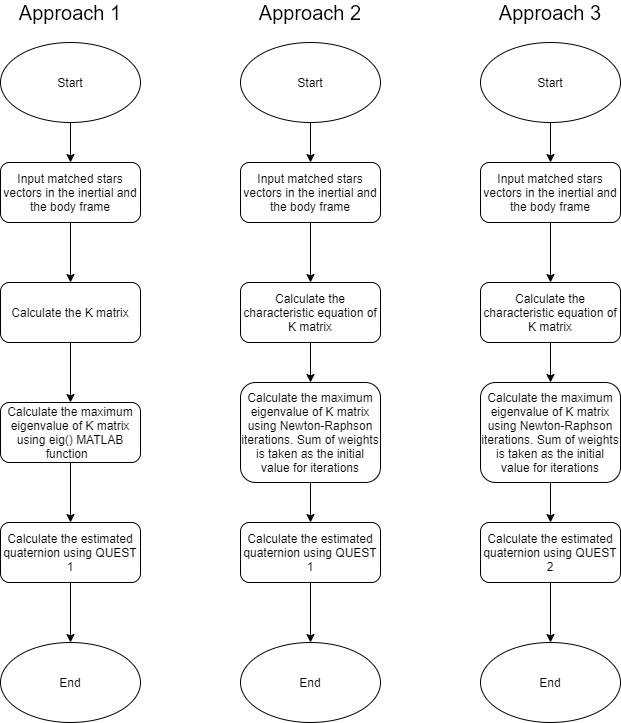
\includegraphics[scale=0.50]{Figures/GNC/estimation_flowchart.png}
\caption{Flow of Code in different Approaches}
\label{sec:esti_flow_of_code}
\end{figure}

}


\subsubsection{Results}
{
Due to the fact that all three implementations of estimation were mathematically identical and there was no limitation on computation cost, the results of the MIL simulation were computed using Approach 2. The requirement for the system is 0.01$^\circ$ (36 arcsec), and since we had to consider a number smaller than our requirements, we set 1 arcsec into the Markley formulas (refer to section \ref{sec:Atti_Accu}) to calculate number of stars. The number of stars were calculated to be ~5.15 which was up scaled to 6. Total of 15 images and a threshold value of 18, 19 and 20 was considered for the simulation. \ref{sec:esti_result_variation} shows plot of error and their norm in each image and their variation as the number of matched stars vary.

\begin{figure}
\centering
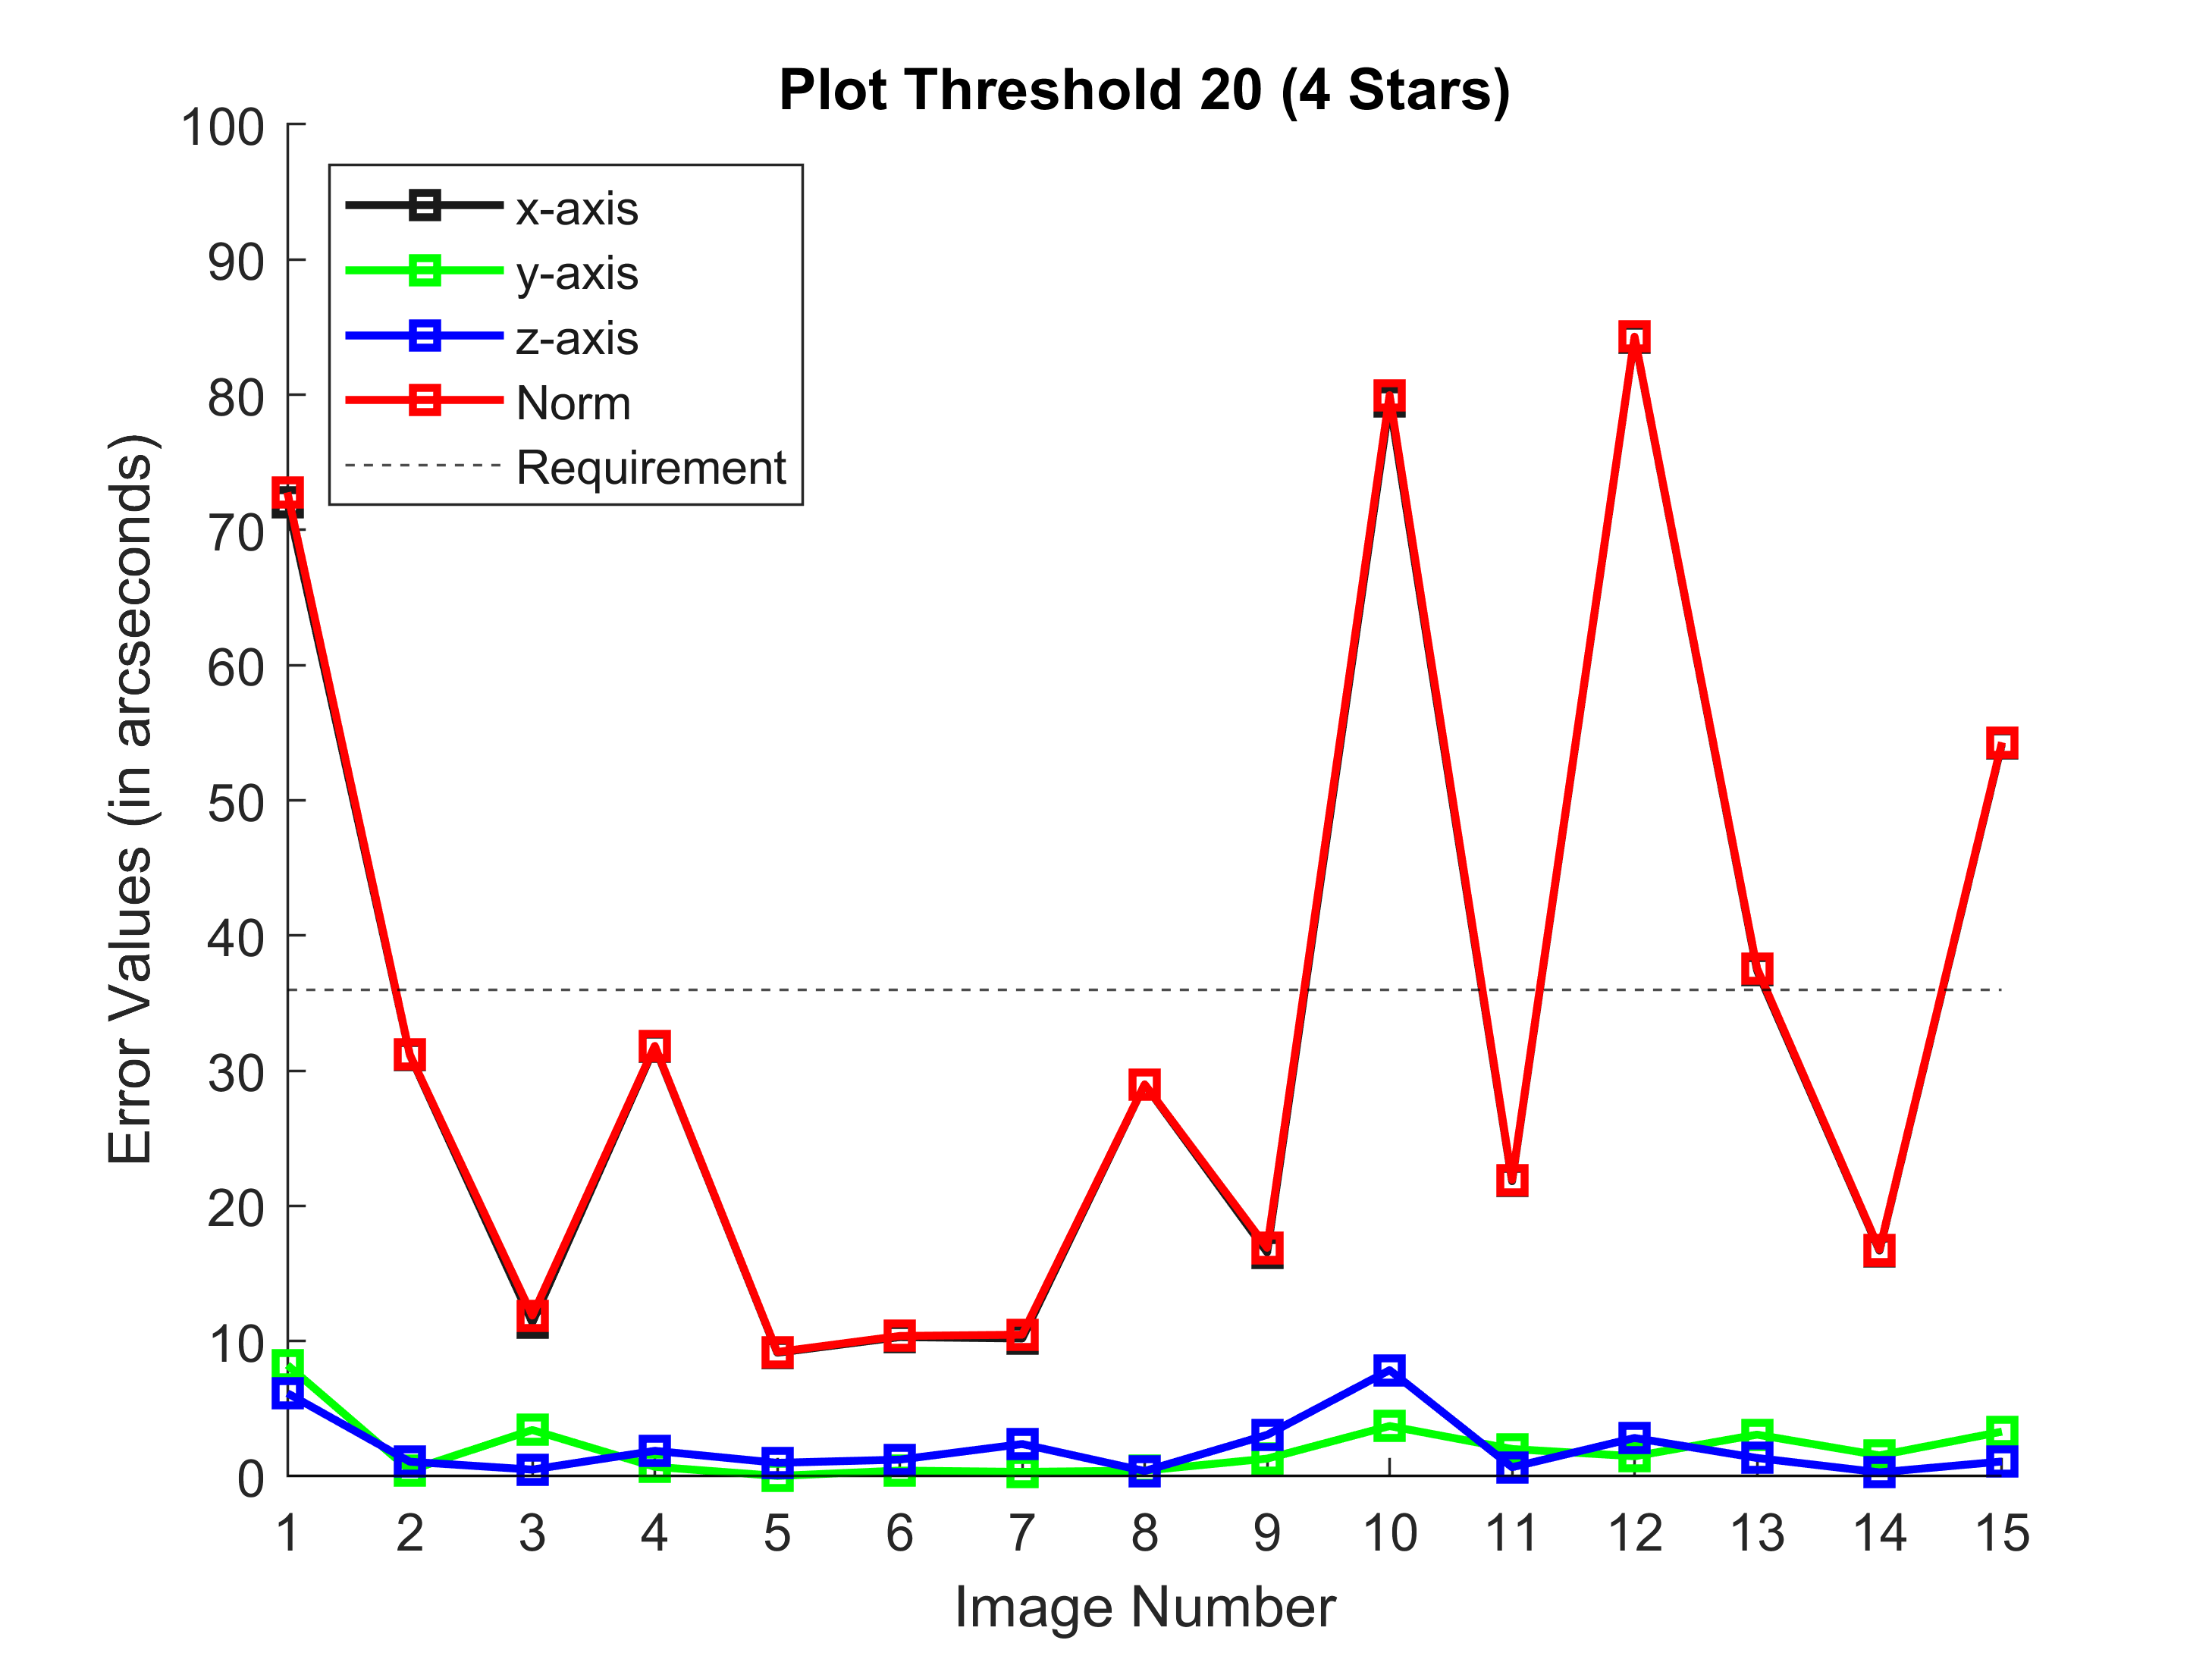
\includegraphics[scale=0.50]{Figures/GNC/Result_Plot_Threshold_20_4stars.png}
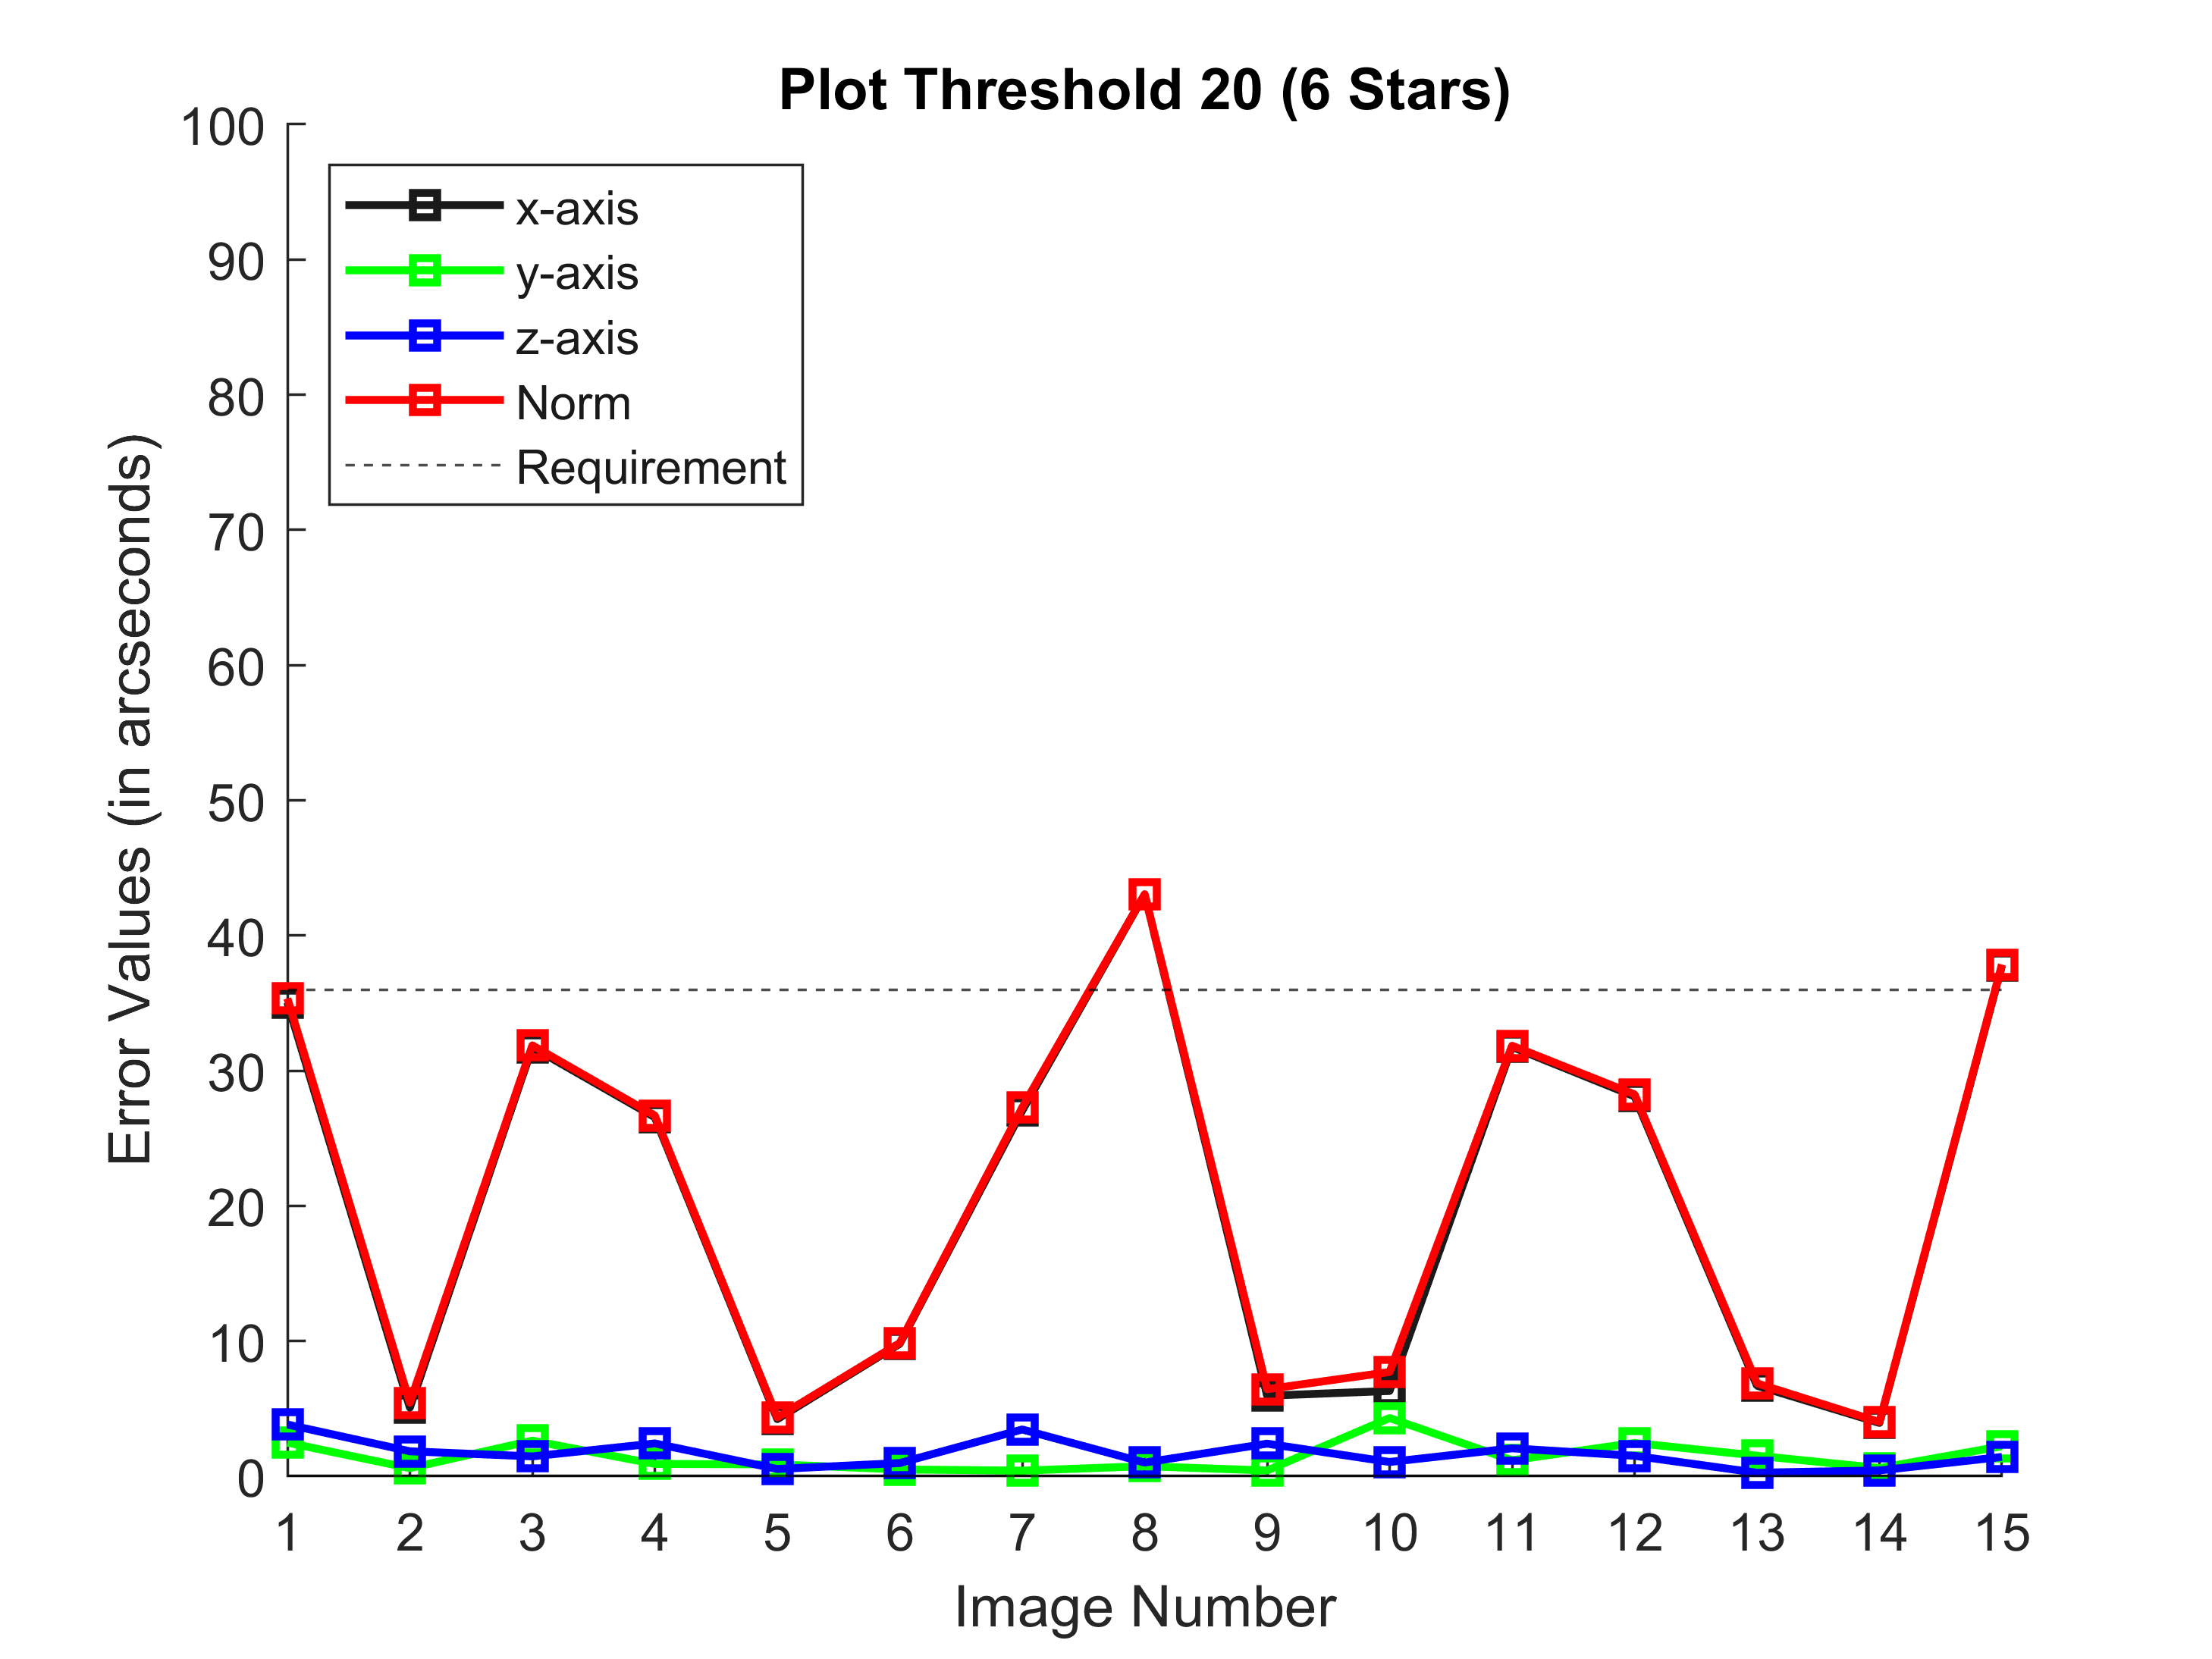
\includegraphics[scale=0.50]{Figures/GNC/Result_Plot_Threshold_20_6stars.png}
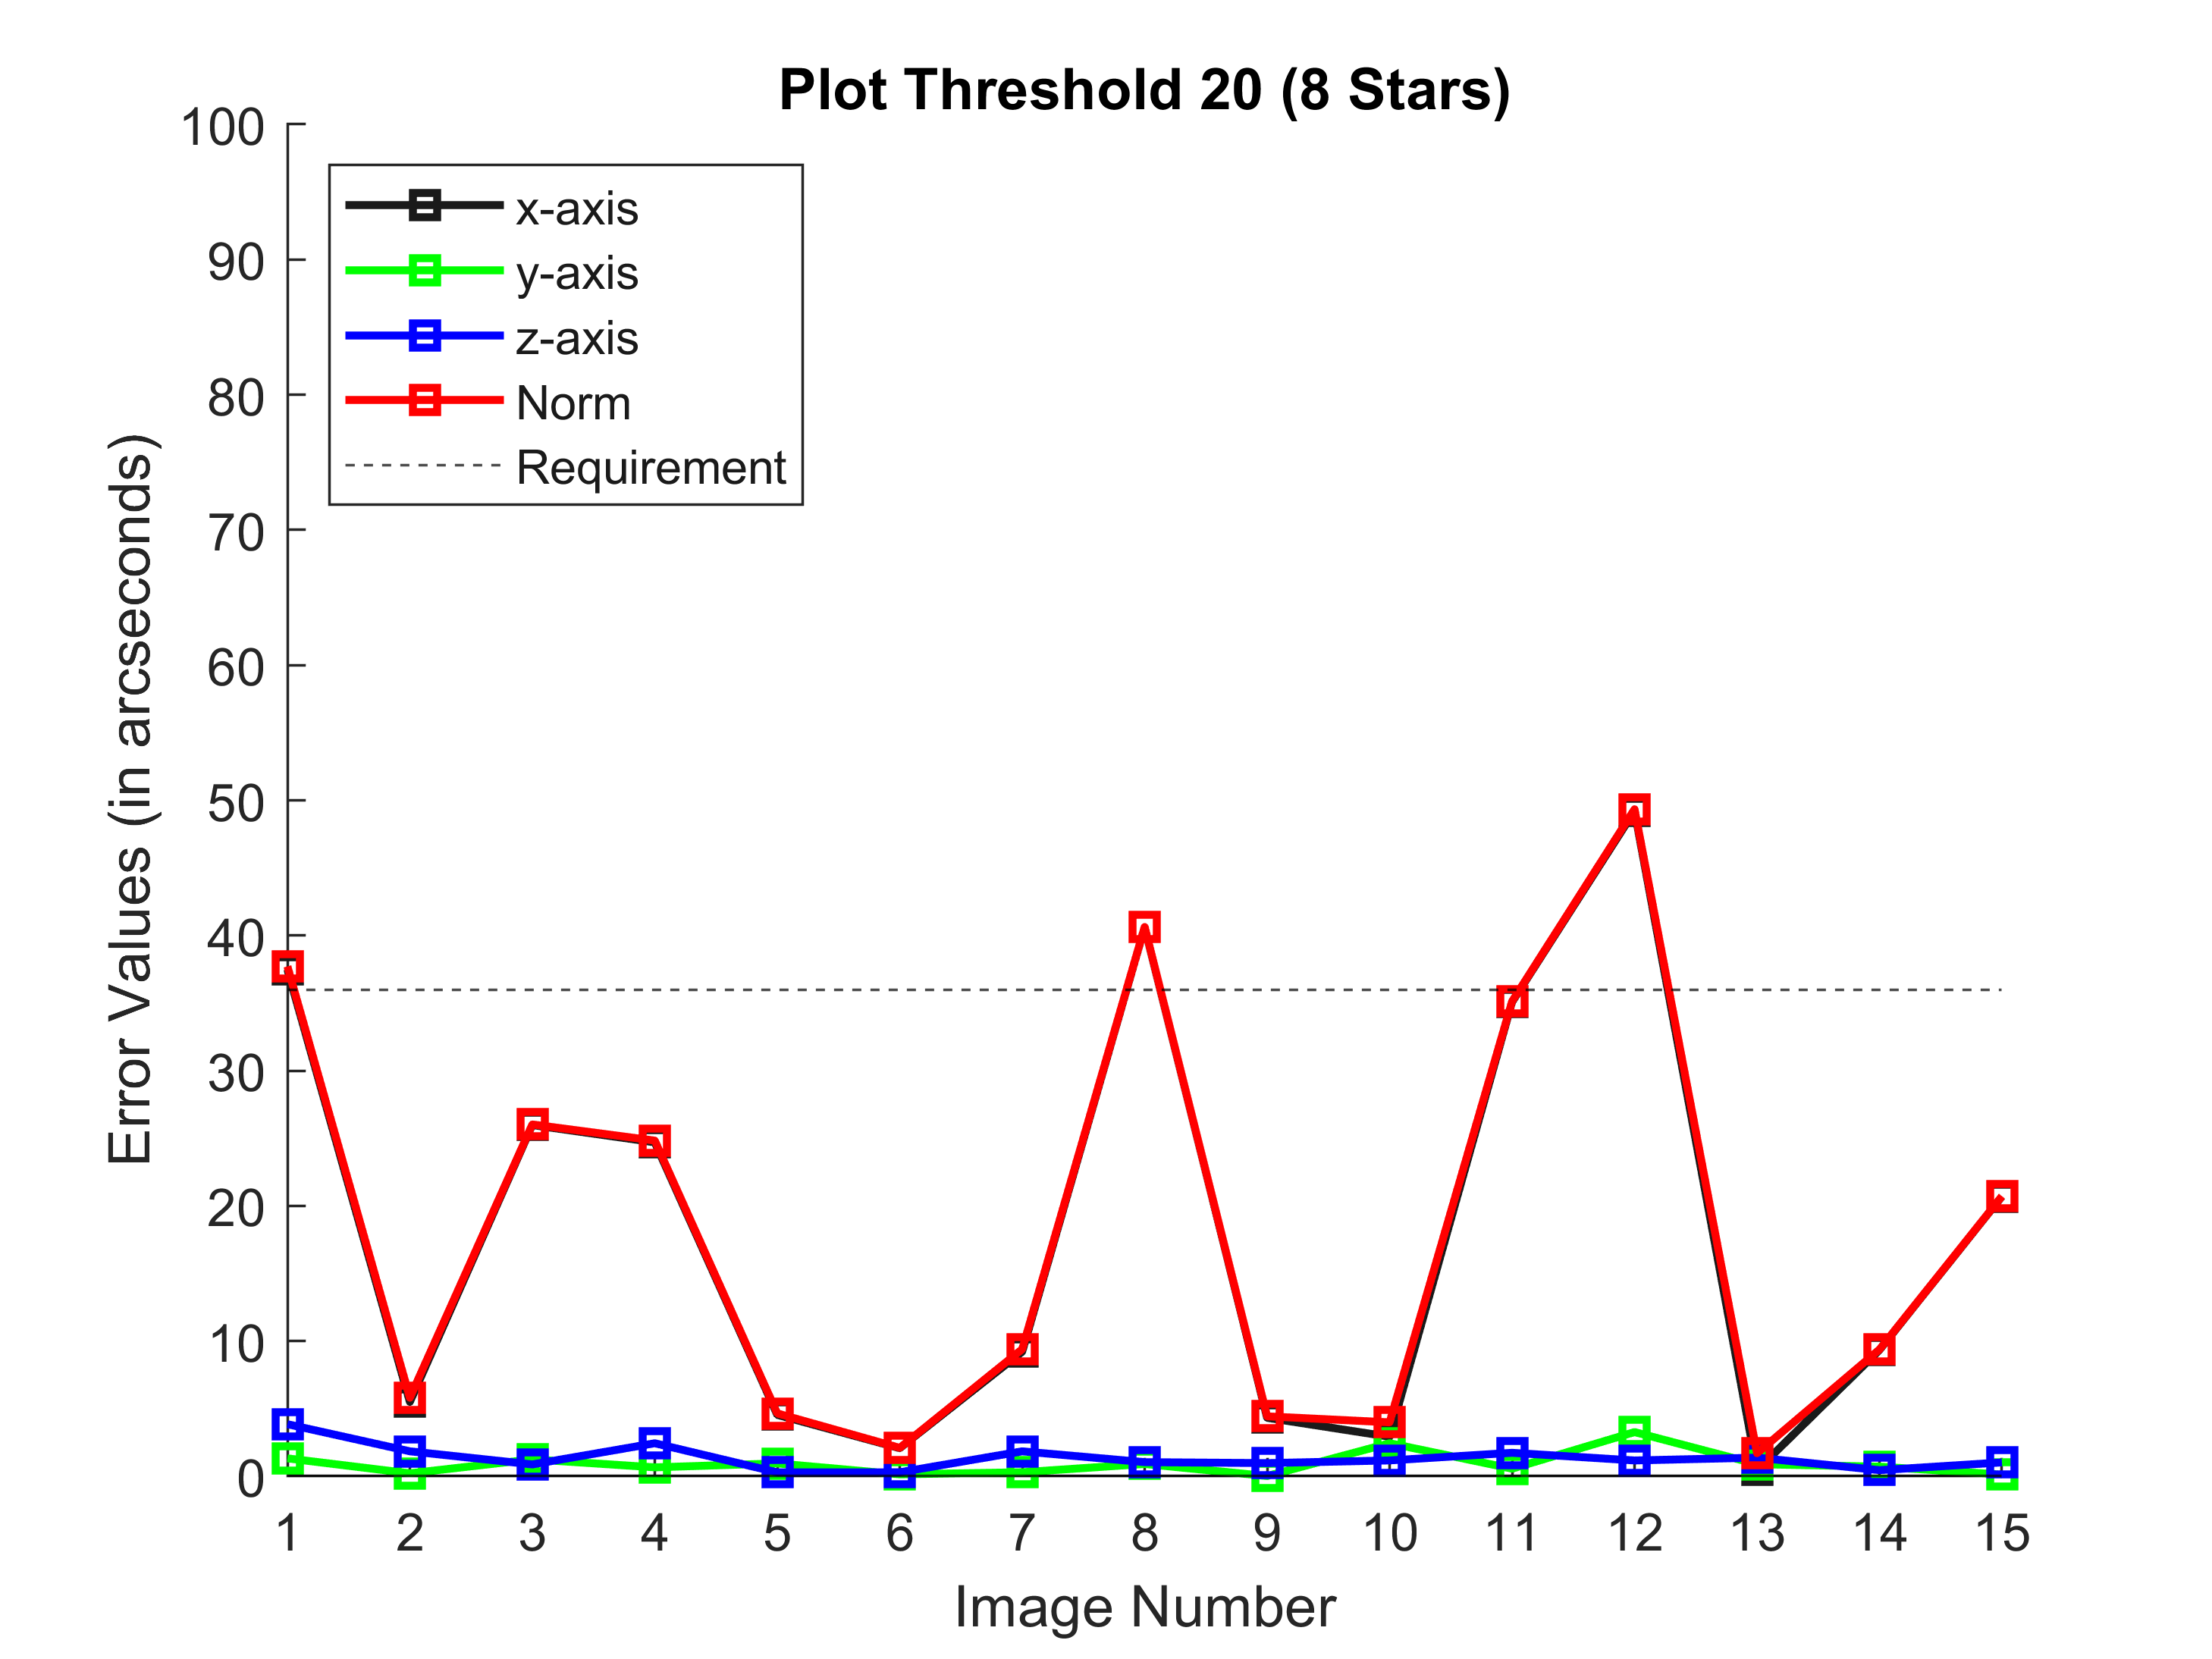
\includegraphics[scale=0.50]{Figures/GNC/Result_Plot_Threshold_20_8stars.png}
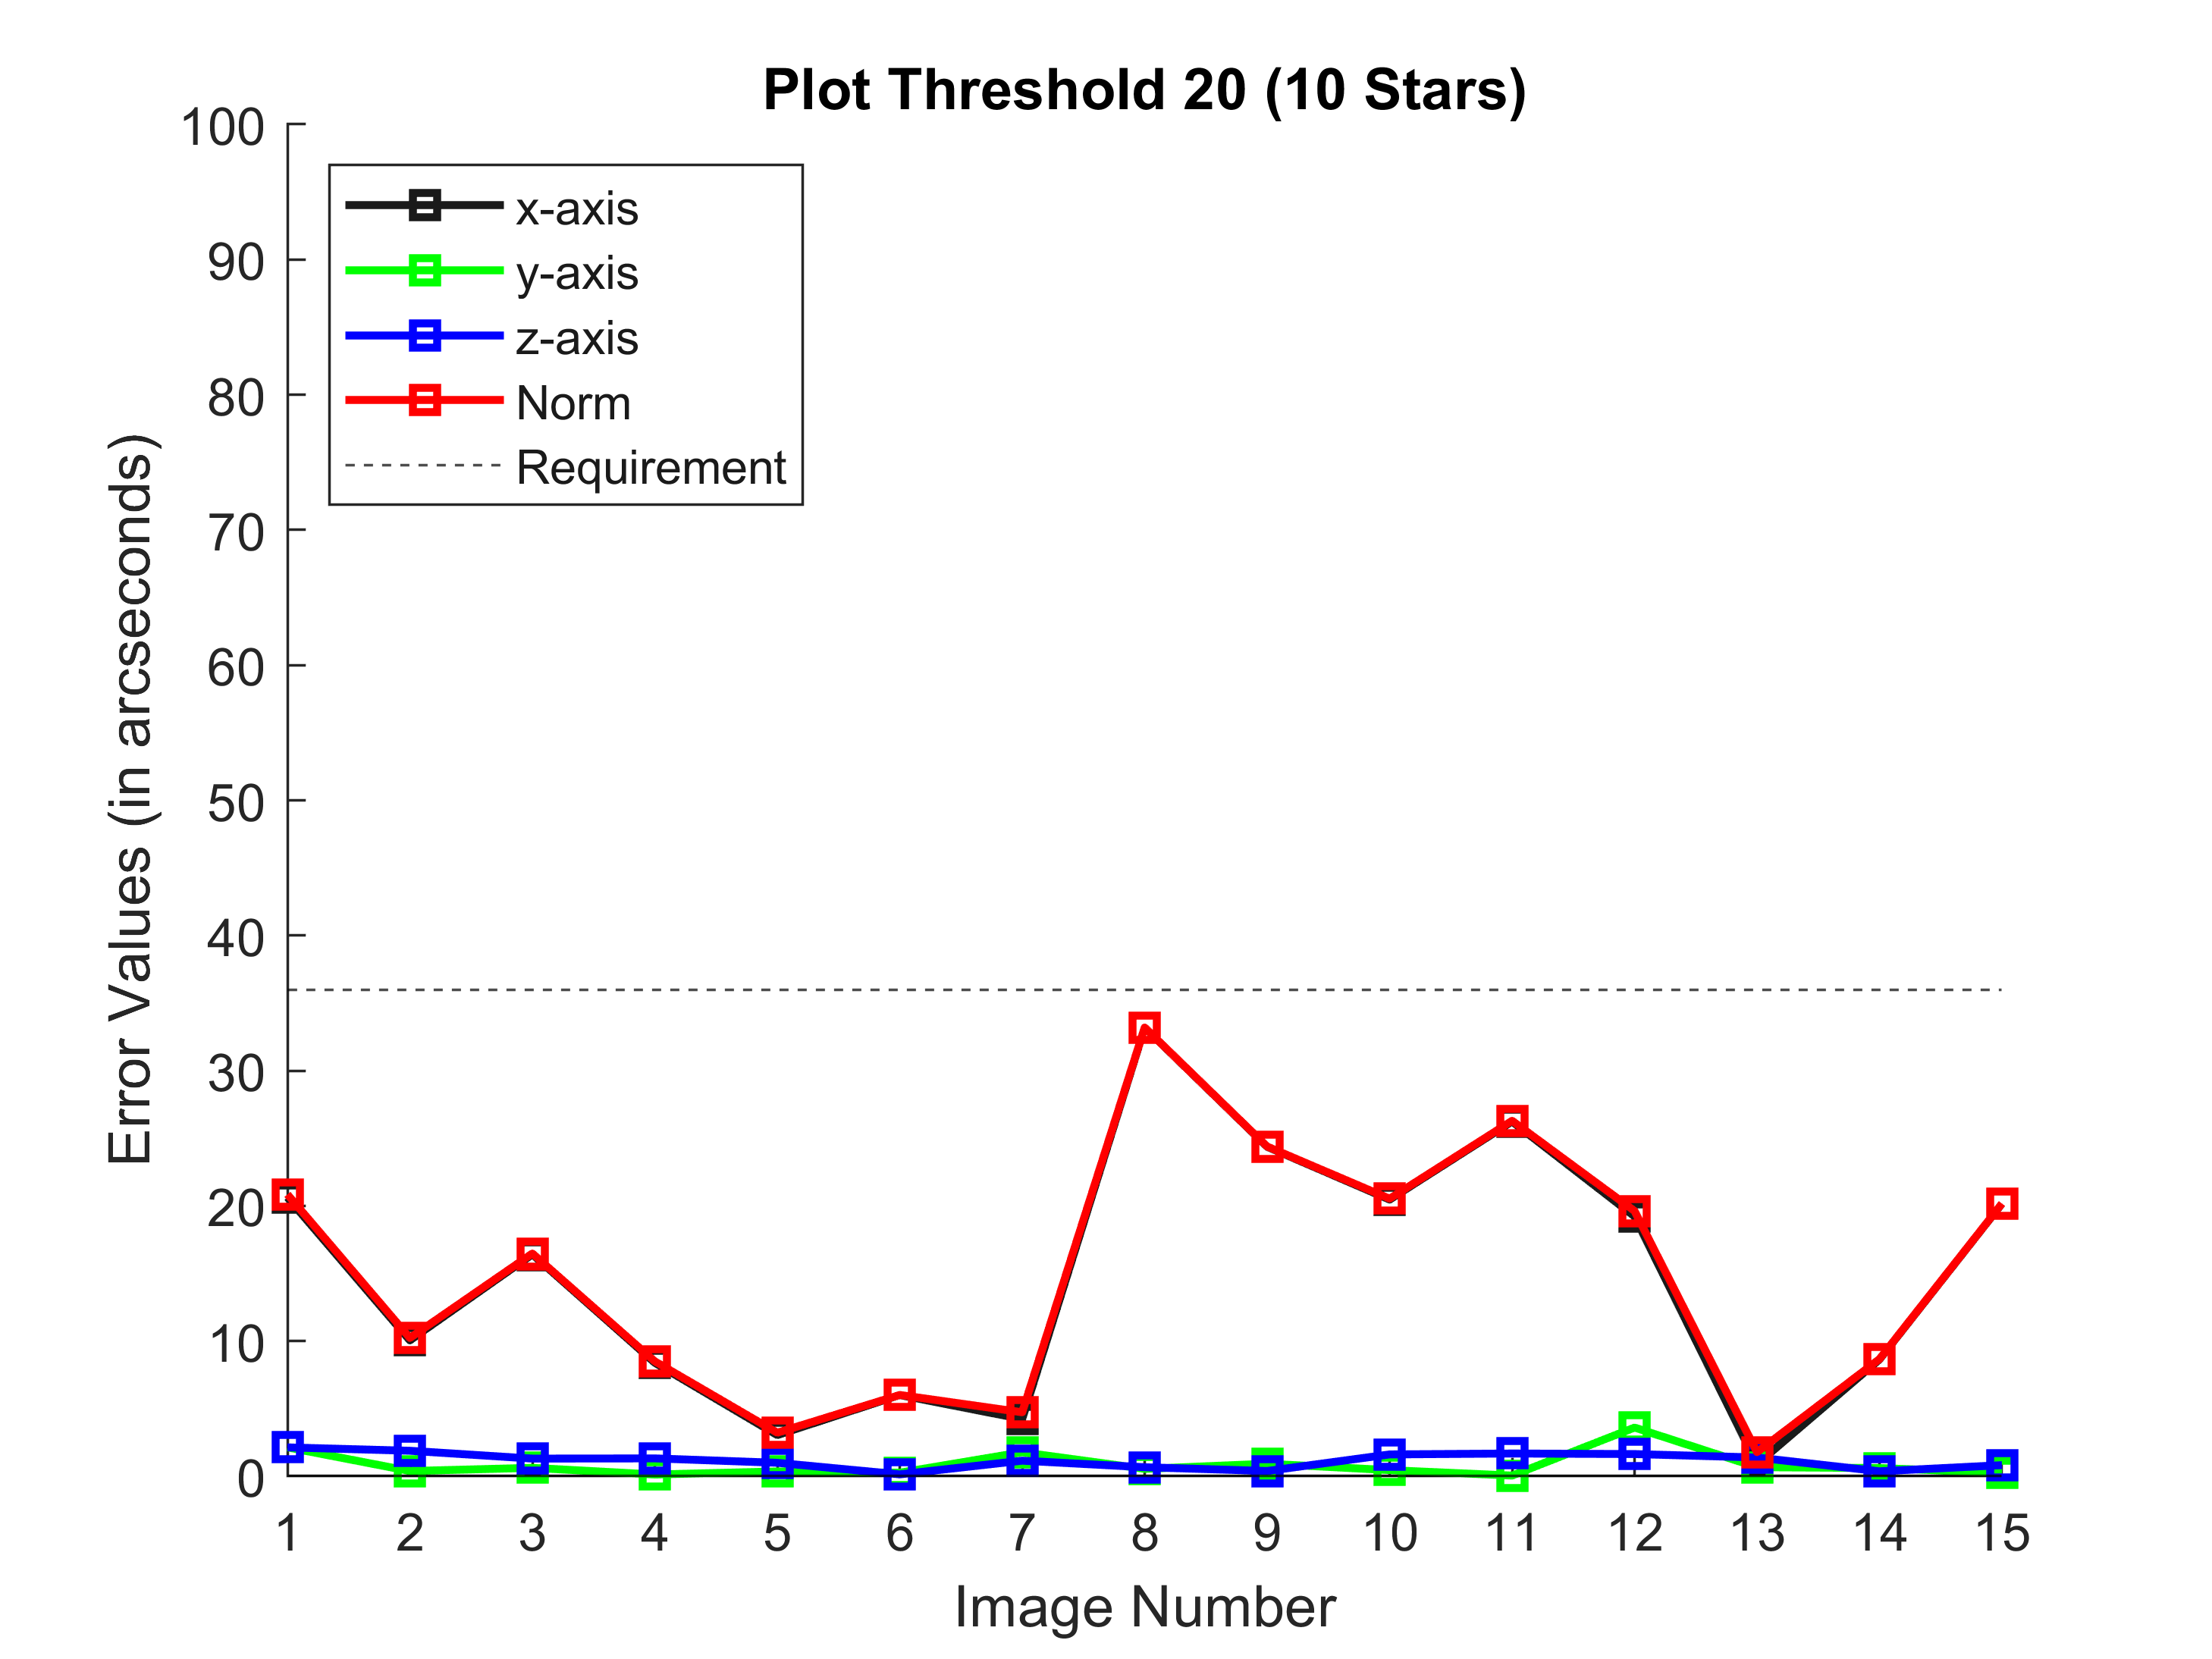
\includegraphics[scale=0.50]{Figures/GNC/Result_Plot_Threshold_20_10stars.png}
\caption{Flow of Code in different Approaches}
\label{sec:esti_result_variation}
\end{figure}
}

}


\subsection{Attitude Accuracy} % Add reference of markley check labels
\label{sec:Atti_Accu}
{
After benchamrking of other star trackers, we set 0.01$^\circ$ (36 arcsec) as accuracy for STADS. From literature survey and benchmarking of other star tracker vendors, we also know that accuracy of a star tracker is defined in terms of certain angles about the their boresight and across boresight axis. We are not clear about the quantities used to express accuracy, more specifically, what are these angles, how do other companies go about calculating them, and what experimental validation do they provide in order to support their values. We will send mails to professors and other companies regarding this issue.

Markley\cite{markley2014fundamentals} provides some insight into accuracy for a star tracker by the following formulas,

Along $X -$direction is -
\begin{equation}
    \Delta \theta_{cross-boresight}^X = \frac{2 \kappa_{cent}^X \beta_{max}^X}{N_{pixels}^X \sqrt{N_{stars}}}
\end{equation}
And along $Y -$direction is -
\begin{equation}
    \Delta \theta_{cross-boresight}^Y = \frac{2 \kappa_{cent}^Y \beta_{max}^Y}{N_{pixels}^Y \sqrt{N_{stars}}}
\end{equation}
The $\kappa_{cent}^{(\cdot)}$ is the maximum centroiding error to obtain the worst case scenario accuracies.
And the Around Boresight Accuracy, or the Roll Accuracy is -
\begin{equation}
    \Delta \theta_{roll} = \frac{\sqrt{6} \kappa_{cent}}{N_{pixels}^* \sqrt{N_{stars}}}
\end{equation}
where,
\begin{equation*}
    N_{pixels}^* = \min\left( N_{pixels}^X, N_{pixels}^Y\right)
\end{equation*}
The lower value of the number of pixels for the rectangular sensor is taken so that the worst-case scenario accuracy is calculated.

The error values in the above formulas, give the maximum achievable accuracy about different axes. For $\kappa_{cent}$ = 0.1 , $N_{pixels}$ = 1024 and $N_{stars}$ = 5, this gives a cross boresight accuracy of 3.1 arcsec for a 20$^\circ$x$20^\circ$ FOV. This means that for these given parameters, the actual accuracy will be greater than or equal to 3.1 arcsec.
Therefore, these set of formulas, only give a lower bound on the achievable error, which doesn't hold any practical significance as the goal of accuracy is to find a upper bound on error. 

These formulas are only helpful to get a rough estimate about the number of stars that must be matched by the star matching algorithm for STADS to have accuracy within the requirements. As these formulas give only the best accuracy, our actual accuracy would be more than this value. So instead of setting accuracy to be 0.01$^\circ$ (36 arcsec) (As in requirements), we set better accuracy than what we intend to achieve in the formulas (We used 1 arcsec for MIL simulation) to find the number of matched stars.

As we didn't have any standard method to quantify error, we came with our own method of quantifying error for the MIL simulation. In this method, error about different axes is defined as the corresponding Euler angles of the error quaternion between actual quaternion and the estimated quaternion.

The error quaternion between 2 quaternions is defined as:
\begin{equation}
    \delta \mathbf{q} \equiv \begin{bmatrix} \mathbf{\delta q_{1:3}} \\ \delta  q_4 \end{bmatrix} = \mathbf{q \otimes \Bar{q}^{-1}}
\end{equation}
where, $\Bar{q}$ is the estimated, and $q$ is the reference quaternion. 

This means that
\begin{equation}
\label{eqn:2}
    \mathbf{\delta q \otimes \bar{q} = q \otimes \bar{q}^{-1} \otimes \bar{q} = q}
\end{equation}
Thus, taking the $\otimes$ product of $\mathbf{\delta q}$ and $\mathbf{\bar{q}}$ gives us $\mathbf{q}$. Thus, $\mathbf{\delta q}$ is the quaternion that takes $\mathbf{\bar{q}}$ to $\mathbf{q}$, as defined in the above equation.

Now here, we can calculate each component of $\mathbf{\delta q}$ as follows:
\begin{align}
     \mathbf{\delta q_{1:3}} = & \,\, \| \mathbf{\bar{q}} \|^{-2} \,\, \mathbf{\Xi(\bar{q})}^T \,\, \mathbf{q = - \| \bar{q} \|}^{-2} \,\, \mathbf{\Xi(q)}^T \,\, \mathbf{\bar{q}} \\ 
     \delta q_4 = & \,\, \| \mathbf{\bar{q}} \|^{-2} \,\, \mathbf{\bar{q}}^T \,\, \mathbf{q}
\end{align}
Where, $\mathbf{\Xi}(\mathbf{q})$ is given by -
\begin{equation}
    \mathbf{\Xi}(\mathbf{q}) = \begin{bmatrix} q_4 & -q_3 & q_2 \\ q_3 & q_4 & -q_1 \\ -q_2 & q_1 & q_4 \\ -q_1 & -q_2 & -q_3 \end{bmatrix}
\end{equation}
Thus, we can evaluate $\delta \mathbf{q}$. 

Therefore the error in the estimated quaternion about x,y,z axes are the corresponding x,y,z Euler angles of the error quaternion, $\delta \mathbf{q}$.

}


}
%----------------------------END----------------------------%
\end{document}